\section{CTCLResult  Class Reference}
\label{classCTCLResult}\index{CTCLResult@{CTCLResult}}
{\tt \#include $<$TCLResult.h$>$}

Inheritance diagram for CTCLResult::\begin{figure}[H]
\begin{center}
\leavevmode
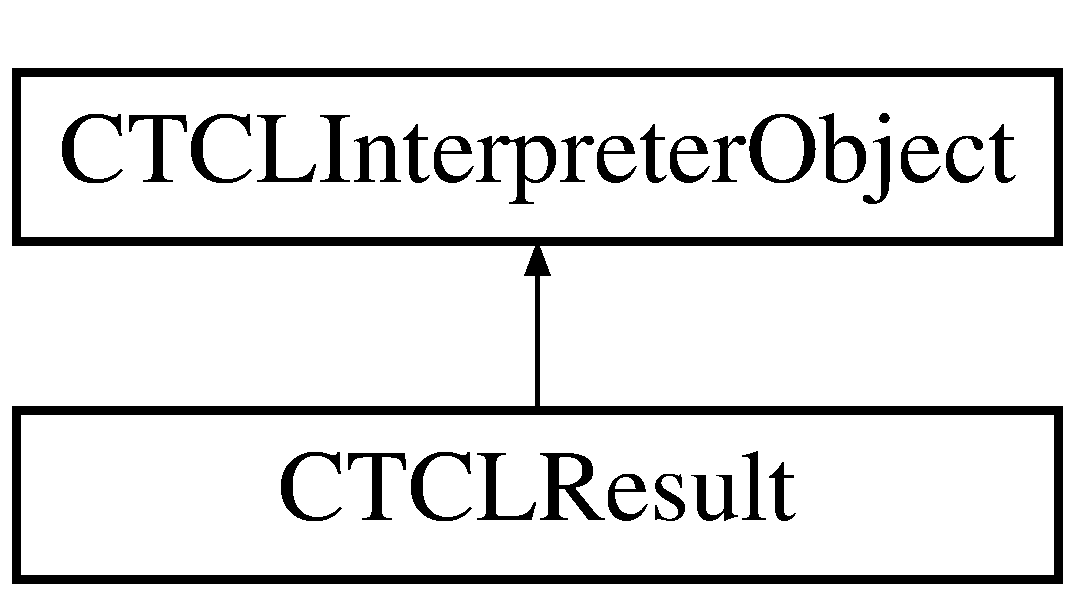
\includegraphics[height=2cm]{classCTCLResult}
\end{center}
\end{figure}
\subsection*{Public Methods}
\begin{CompactItemize}
\item 
{\bf CTCLResult} ()
\item 
{\bf $\sim$CTCLResult} ()
\item 
{\bf CTCLResult} ({\bf CTCLInterpreter} $\ast$p\-Interp)
\item 
{\bf CTCLResult} (const CTCLResult \&a\-CTCLResult)
\item 
CTCLResult \& {\bf operator=} (const CTCLResult \&a\-CTCLResult)
\item 
int {\bf operator==} (const CTCLResult \&a\-CTCLResult)
\item 
CTCLResult \& {\bf operator=} (const char $\ast$p\-String)
\item 
CTCLResult \& {\bf operator=} (const std::string \&r\-String)
\item 
CTCLResult \& {\bf operator+=} (const char $\ast$p\-String)
\item 
CTCLResult \& {\bf operator+=} (const std::string \&r\-String)
\item 
CTCLResult \& {\bf operator+} (const char $\ast$p\-String)
\item 
CTCLResult \& {\bf operator+} (const std::string \&r\-String)
\item 
void {\bf Clear} ()
\item 
void {\bf Append\-Element} (const char $\ast$p\-String)
\item 
void {\bf Append\-Element} (const std::string \&r\-String)
\item 
{\bf operator const char $\ast$} ()
\item 
{\bf operator std::string} ()
\item 
{\bf operator CTCLString} ()
\end{CompactItemize}


\subsection{Constructor \& Destructor Documentation}
\index{CTCLResult@{CTCLResult}!CTCLResult@{CTCLResult}}
\index{CTCLResult@{CTCLResult}!CTCLResult@{CTCLResult}}
\subsubsection{\setlength{\rightskip}{0pt plus 5cm}CTCLResult::CTCLResult ()\hspace{0.3cm}{\tt  [inline]}}\label{classCTCLResult_a0}




Definition at line 315 of file TCLResult.h.\index{CTCLResult@{CTCLResult}!~CTCLResult@{$\sim$CTCLResult}}
\index{~CTCLResult@{$\sim$CTCLResult}!CTCLResult@{CTCLResult}}
\subsubsection{\setlength{\rightskip}{0pt plus 5cm}CTCLResult::$\sim$CTCLResult ()\hspace{0.3cm}{\tt  [inline]}}\label{classCTCLResult_a1}




Definition at line 316 of file TCLResult.h.\index{CTCLResult@{CTCLResult}!CTCLResult@{CTCLResult}}
\index{CTCLResult@{CTCLResult}!CTCLResult@{CTCLResult}}
\subsubsection{\setlength{\rightskip}{0pt plus 5cm}CTCLResult::CTCLResult ({\bf CTCLInterpreter} $\ast$ {\em p\-Interp})\hspace{0.3cm}{\tt  [inline]}}\label{classCTCLResult_a2}




Definition at line 320 of file TCLResult.h.\index{CTCLResult@{CTCLResult}!CTCLResult@{CTCLResult}}
\index{CTCLResult@{CTCLResult}!CTCLResult@{CTCLResult}}
\subsubsection{\setlength{\rightskip}{0pt plus 5cm}CTCLResult::CTCLResult (const CTCLResult \& {\em a\-CTCLResult})\hspace{0.3cm}{\tt  [inline]}}\label{classCTCLResult_a3}




Definition at line 326 of file TCLResult.h.

\subsection{Member Function Documentation}
\index{CTCLResult@{CTCLResult}!AppendElement@{AppendElement}}
\index{AppendElement@{AppendElement}!CTCLResult@{CTCLResult}}
\subsubsection{\setlength{\rightskip}{0pt plus 5cm}void CTCLResult::Append\-Element (const std::string \& {\em r\-String})\hspace{0.3cm}{\tt  [inline]}}\label{classCTCLResult_a14}




Definition at line 373 of file TCLResult.h.

References Append\-Element().\index{CTCLResult@{CTCLResult}!AppendElement@{AppendElement}}
\index{AppendElement@{AppendElement}!CTCLResult@{CTCLResult}}
\subsubsection{\setlength{\rightskip}{0pt plus 5cm}void CTCLResult::Append\-Element (const char $\ast$ {\em p\-String})}\label{classCTCLResult_a13}




Definition at line 394 of file TCLResult.cpp.

References CTCLInterpreter\-Object::Assert\-If\-Not\-Bound(), and CTCLInterpreter::get\-Interpreter().

Referenced by Append\-Element().\index{CTCLResult@{CTCLResult}!Clear@{Clear}}
\index{Clear@{Clear}!CTCLResult@{CTCLResult}}
\subsubsection{\setlength{\rightskip}{0pt plus 5cm}void CTCLResult::Clear ()}\label{classCTCLResult_a12}




Definition at line 377 of file TCLResult.cpp.

References CTCLInterpreter\-Object::Assert\-If\-Not\-Bound(), and CTCLInterpreter::get\-Interpreter().\index{CTCLResult@{CTCLResult}!operator const char *@{operator const char $\ast$}}
\index{operator const char *@{operator const char $\ast$}!CTCLResult@{CTCLResult}}
\subsubsection{\setlength{\rightskip}{0pt plus 5cm}CTCLResult::operator const char $\ast$ ()}\label{classCTCLResult_a15}




Definition at line 417 of file TCLResult.cpp.

References CTCLInterpreter\-Object::Assert\-If\-Not\-Bound(), and CTCLInterpreter::get\-Interpreter().\index{CTCLResult@{CTCLResult}!operator CTCLString@{operator CTCLString}}
\index{operator CTCLString@{operator CTCLString}!CTCLResult@{CTCLResult}}
\subsubsection{\setlength{\rightskip}{0pt plus 5cm}CTCLResult::operator {\bf CTCLString} ()}\label{classCTCLResult_a17}




Definition at line 450 of file TCLResult.cpp.\index{CTCLResult@{CTCLResult}!operator std::string@{operator std::string}}
\index{operator std::string@{operator std::string}!CTCLResult@{CTCLResult}}
\subsubsection{\setlength{\rightskip}{0pt plus 5cm}CTCLResult::operator std::string ()}\label{classCTCLResult_a16}




Definition at line 434 of file TCLResult.cpp.\index{CTCLResult@{CTCLResult}!operator+@{operator+}}
\index{operator+@{operator+}!CTCLResult@{CTCLResult}}
\subsubsection{\setlength{\rightskip}{0pt plus 5cm}CTCLResult\& CTCLResult::operator+ (const std::string \& {\em r\-String})\hspace{0.3cm}{\tt  [inline]}}\label{classCTCLResult_a11}




Definition at line 366 of file TCLResult.h.

References operator+=().\index{CTCLResult@{CTCLResult}!operator+@{operator+}}
\index{operator+@{operator+}!CTCLResult@{CTCLResult}}
\subsubsection{\setlength{\rightskip}{0pt plus 5cm}CTCLResult\& CTCLResult::operator+ (const char $\ast$ {\em p\-String})\hspace{0.3cm}{\tt  [inline]}}\label{classCTCLResult_a10}




Definition at line 363 of file TCLResult.h.

References operator+=().\index{CTCLResult@{CTCLResult}!operator+=@{operator+=}}
\index{operator+=@{operator+=}!CTCLResult@{CTCLResult}}
\subsubsection{\setlength{\rightskip}{0pt plus 5cm}CTCLResult\& CTCLResult::operator+= (const std::string \& {\em r\-String})\hspace{0.3cm}{\tt  [inline]}}\label{classCTCLResult_a9}




Definition at line 360 of file TCLResult.h.

References operator+=().\index{CTCLResult@{CTCLResult}!operator+=@{operator+=}}
\index{operator+=@{operator+=}!CTCLResult@{CTCLResult}}
\subsubsection{\setlength{\rightskip}{0pt plus 5cm}CTCLResult \& CTCLResult::operator+= (const char $\ast$ {\em p\-String})}\label{classCTCLResult_a8}




Definition at line 350 of file TCLResult.cpp.

References CTCLInterpreter\-Object::Assert\-If\-Not\-Bound(), and CTCLInterpreter::get\-Interpreter().

Referenced by operator+(), and operator+=().\index{CTCLResult@{CTCLResult}!operator=@{operator=}}
\index{operator=@{operator=}!CTCLResult@{CTCLResult}}
\subsubsection{\setlength{\rightskip}{0pt plus 5cm}CTCLResult\& CTCLResult::operator= (const std::string \& {\em r\-String})\hspace{0.3cm}{\tt  [inline]}}\label{classCTCLResult_a7}




Definition at line 355 of file TCLResult.h.

References operator=().\index{CTCLResult@{CTCLResult}!operator=@{operator=}}
\index{operator=@{operator=}!CTCLResult@{CTCLResult}}
\subsubsection{\setlength{\rightskip}{0pt plus 5cm}CTCLResult \& CTCLResult::operator= (const char $\ast$ {\em p\-String})}\label{classCTCLResult_a6}




Definition at line 321 of file TCLResult.cpp.

References CTCLInterpreter\-Object::Assert\-If\-Not\-Bound(), and CTCLInterpreter::get\-Interpreter().\index{CTCLResult@{CTCLResult}!operator=@{operator=}}
\index{operator=@{operator=}!CTCLResult@{CTCLResult}}
\subsubsection{\setlength{\rightskip}{0pt plus 5cm}CTCLResult\& CTCLResult::operator= (const CTCLResult \& {\em a\-CTCLResult})\hspace{0.3cm}{\tt  [inline]}}\label{classCTCLResult_a4}




Definition at line 334 of file TCLResult.h.

References CTCLInterpreter\-Object::operator=().

Referenced by operator=().\index{CTCLResult@{CTCLResult}!operator==@{operator==}}
\index{operator==@{operator==}!CTCLResult@{CTCLResult}}
\subsubsection{\setlength{\rightskip}{0pt plus 5cm}int CTCLResult::operator== (const CTCLResult \& {\em a\-CTCLResult})\hspace{0.3cm}{\tt  [inline]}}\label{classCTCLResult_a5}




Definition at line 344 of file TCLResult.h.

References CTCLInterpreter\-Object::operator==().

The documentation for this class was generated from the following files:\begin{CompactItemize}
\item 
{\bf TCLResult.h}\item 
{\bf TCLResult.cpp}\end{CompactItemize}
